
%%%%%%%%%%%%%%%%%%%%%%%%%%%%%%%%%%%%%%%%%%%%%%%%%%%%%%%%%%%%%%%%%%%%%%%
\subsection{Statistische Netzwerkanalyse}
%%%%%%%%%%%%%%%%%%%%%%%%%%%%%%%%%%%%%%%%%%%%%%%%%%%%%%%%%%%%%%%%%%%%%%%
\begin{frame}
\frametitle{Probing}
\framesubtitle{Korrelierung von Netzwerkscans}

\begin{alertblock}{\textit{scanning detection systems}}
    \begin{itemize}
        \item Trafficanalyse zu ungenau
        \item Erstellung eines \textit{fingerprints} kaum möglich
    \end{itemize}
\end{alertblock}

\begin{exampleblock}{\textit{Verkehrskorrelation durch statistische Verfahren}}
    \begin{itemize}
        \item Scans werden zeitlich korreliert
        \item Scan-Traffic zuordnung zu Scan-Technik
    \end{itemize}
\end{exampleblock}

\end{frame}
\begin{frame}
\frametitle{Probing}
\framesubtitle{Korrelierung von Netzwerkscans}

\begin{center}
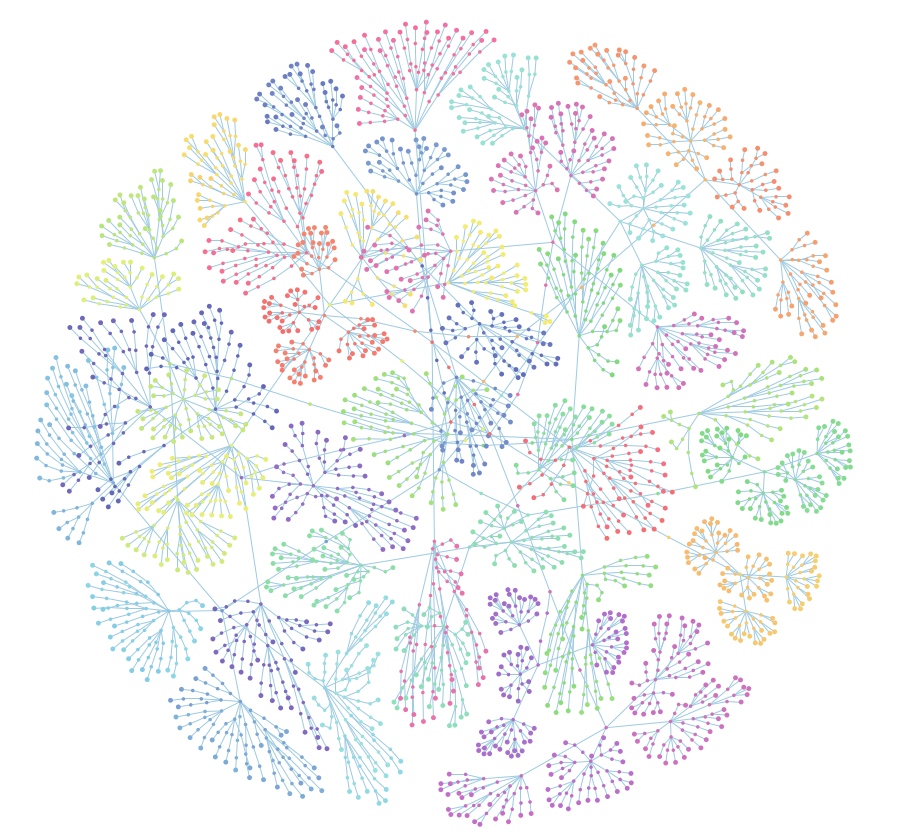
\includegraphics[scale=0.23]{img/statistical_network_analysis.png}
\end{center}



\vspace{0.5cm}

\footnoterule
\footnotesize{
    Quelle:
    Bou-Harb, E., Debbabi, M., \& Assi, C. (2014) Behavioral analytics for inferring
    large-scale orchestrated probing events. In 2014 IEEE Conference on Computer 
    Communications Workshops (INFOCOM WKSHPS) (pp. 506–511). New York, NY: IEEE.
}


\end{frame}

